\section{ExternalModel plugins}
\label{sec:newExternalModelPlugin}
\begin{figure}
\centering
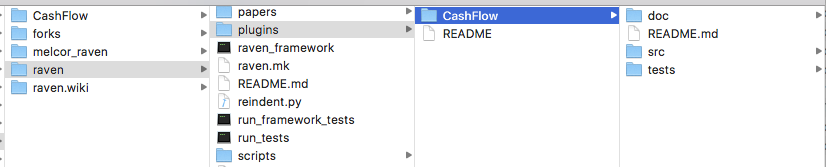
\includegraphics[width=1.0\textwidth]{pics/plugins_location.png}
\caption{Plugins Location}
\label{fig:pluginsLocation}
\end{figure}
The procedure of adding a plugin for the ExternalModel is a straightforward  process.
The addition of a plugin does not require modifying RAVEN itself.
Instead, the developer creates a new Python module that is going to be embedded
 in RAVEN at run-time (no need to introduce  hard-coded statements).
 This plugin needs to be placed in a folder (whatever name) located in (see figure~\ref{fig:pluginsLocation}):
\begin{lstlisting}[language=bash]
 path/to/raven/plugins/
\end{lstlisting}
In order to install a new plugin, the user can run the script contained in the RAVEN script folder:
\begin{lstlisting}[language=bash]
 python path/to/raven/scripts/install_plugins.py  **directory**
\end{lstlisting}
where  $**directory**$ should be replaced with the absolute path to the plugin directory.
(e.g. ``path/to/my/plugins/folder''). If the plugin developer wants to make of his plugin
an official supported plugin in RAVEN (by the submodule system), he needs to check
the raven wiki under the ``contribution'' section).

At the initialization stage, RAVEN imports all the Plugins that are contained in this directory and performs some preliminary cross-checks.
\\It is important to notice that the name of class in the Plugin module is the one the user needs to specify when the new plugin
needs to be used. For example, if the Plugin module contains the class 	``NewPlugin'', the \textit{subType} in the \xmlNode{ExternalModel} block will be 	``NewPlugin'':
\begin{lstlisting}[language=python]
  class NewPlugin(ExternalModelPluginBase):
    ...
\end{lstlisting}
\begin{lstlisting}[style=XML,morekeywords={name,file}] %moreemph={name,file}]
  <Models>
    ...
    <ExternalModel name='whatever' subType='NewPlugin'>
     ...
    </ExternalModel>
    ...
  </Models>
\end{lstlisting}

In the following sub-sections, a step-by-step procedure for creating a new ExternalModel plugin is outlined.

\subsection{ExternalModel Plugin Input}
\label{subsec:externalModelPluginInput}
When a new ExternalModel plugin is developed, its RAVEN input is almost identical
to the general ExternalModel entity (see \ref{subsec:models_externalModel}).
The specifications of an ExternalModel Plugin must be defined within the XML block
\xmlNode{ExternalModel}.
%
This XML node needs to contain the attributes:

\vspace{-5mm}
\begin{itemize}
  \itemsep0em
  \item \xmlAttr{name}, \xmlDesc{required string attribute}, user-defined name
  of this External Model.
  %
  \nb As with the other objects, this is the name that can be used to refer to
  this specific entity from other input blocks in the XML.
  \item \xmlAttr{subType}, \xmlDesc{required string attribute}, must be equal to the
  name of the new plugin the user wants to use (e.g. $NewPlugin$).
  \nb In case a plugin is requested (through the  \xmlAttr{subType} attribute) the
  attribute \xmlAttr{ModuleToLoad} must not be inputted.
  %
\end{itemize}
\vspace{-5mm}

In order to make the RAVEN code aware of the variables the user is going to
manipulate/use in her/his ExternalModel Plugin, the variables need to be specified
in the \xmlNode{ExternalModel} input block.
%
The user needs to input, within this block, only the variables that RAVEN needs
to be aware of (i.e. the variables are going to directly be used by the Plugin)
and not the local variables that the ExternalModel Plugin developer does not want to,
for example, store in a RAVEN internal object.
%
These variables are specified within a \xmlNode{variables} block:
\begin{itemize}
  \item \xmlNode{variables}, \xmlDesc{string, required parameter}.
  %
  Comma-separated list of variable names.
  %
  Each variable name needs to match a variable used/defined in the external python
  model.
  %
\end{itemize}

In addition, if the user wants to use the alias system, the following XML block can be used as
described in the RAVEN user manual under Models.

When the Plugin variables are defined, at run time, RAVEN initializes
them and tracks their values during the simulation.
%
Each variable defined in the \xmlNode{ExternalModel} block is available in the
Plugin class (in each implemented method ) as the object ``container'' that ``acts''
as a Python ``self''. For example,
\begin{lstlisting}[language=python]
  def run (self, container, inputs):
    print(container.variableA)
\end{lstlisting}

%%%%%%%
\subsection{ExternalModel Plugin Creation}
\label{subsec:externalModelPluginCreation}
As already mentioned, RAVEN imports all the ``ExternalModel Plugins'' at run-time.
In order to make RAVEN
able to drive a newer ExternalModel plugin, the developer needs to code a Python class
containing few methods (with strict syntax) that are called by RAVEN during the simulation.
\\ Every new ``ExternalModel Plugin'' must inherit from a RAVEN base class named
$ExternalModelPluginBase$:
\begin{lstlisting}[language=python]
  class NewPlugin(ExternalModelPluginBase):
    ...
\end{lstlisting}
This base class is needed by RAVEN to identify in the plugins folder which class must
be considered an  ``ExternalModel Plugin''.
\\ In addition, when loading an ``ExternalModel Plugin'', RAVEN expects to find, in the class representing the plugin,
 the following required methods:
\begin{lstlisting}[language=python]
from ExternalModelPluginBase import ExternalModelPluginBase
class NewPlugin(ExternalModelPluginBase):
  def run (self, container, Inputs)
\end{lstlisting}
In addition, the following optional methods can be specified:
\begin{lstlisting}[language=python]
from ExternalModelPluginBase import ExternalModelPluginBase
class NewPlugin(ExternalModelPluginBase):
  ...
  def createNewInput(self, container, inputs, samplerType, **Kwargs)
  def _readMoreXML(self, container, xmlNode)
  def initialize(self,container, runInfo, inputs)
\end{lstlisting}
In the following sub-sections all the methods are fully explained, providing examples.
\subsubsection{Method: \texttt{run}}
\label{subsubsec:runExternalModelPlugin}
\begin{lstlisting}[language=python]
def run (self, container, Inputs)
\end{lstlisting}
As stated previously, the only method that \emph{must} be present in an
ExternalModel Plugin is the \textbf{run} function.
%
In this function, the plugin developer needs to implement the algorithm that RAVEN will
execute.
%
The \texttt{\textbf{run}} method is generally called after having inquired the
``createNewInput'' method (either the internal RAVEN one or the one implemented by
the plugin developer).
%
The only two attributes this method is going to receive are a Python list of inputs
(the inputs coming from the \texttt{createNewInput} method) and a ``self-like'' object
named ``container''.
%
If the user wants RAVEN to collect the results of this method, the outcomes of
interest need to be stored in the above mentioned ``container'' object.
%
\nb RAVEN is trying to collect the values of the variables listed only in the
\xmlNode{ExternalModel} XML block.
%
In the following an example is reported:
\begin{lstlisting}[language=python]
def run(self, container, Input):
  # in here the actual run of the
  # model is implemented
  input = Input[0]
  container.outcome = container.sigma*container.rho*input[``whatEver'']
\end{lstlisting}

\subsubsection{Method: \texttt{createNewInput}}
\label{subsubsec:createNewInputExternalModelPlugin}
\begin{lstlisting}[language=python]
def createNewInput(self, container, inputs, samplerType, **Kwargs)
\end{lstlisting}

The \textbf{createNewInput} method can be implemented by the ExternalModel Plugin
developer to create a new input with the information coming from the RAVEN framework.
%
In this function, the developer can retrieve the information coming from the RAVEN
framework, during the employment of a calculation flow, and use them to
construct a new input that is going to be transferred to the ``run'' method.
%
The new input created needs to be returned to RAVEN (i.e. ``return NewInput'').
\\This method expects that the new input is returned in a Python ``dictionary''.
%
RAVEN communicates, thorough a set of method attributes, all the information
that are generally needed to create a new input:

\begin{itemize}
  \item \texttt{inputs}, \xmlDesc{python list}, a list of all the inputs that
  have been defined in the ``Step'' using this model.
  \item \texttt{samplerType}, \xmlDesc{string}, the type of Sampler, if a
  sampling strategy is employed; will be None otherwise.
  \item \texttt{Kwargs}, \xmlDesc{dictionary}, a dictionary containing several
  pieces of information (that can change based on the ``Step'' type).
  %
  If a sampling strategy is employed, this dictionary contains another
  dictionary identified by the keyword ``SampledVars'', in which the variables
  perturbed by the sampler are reported.
\end{itemize}
\nb If the ``Step'' that is using this Model has as input(s) an object of main
class type ``DataObjects'' (see Section~\ref{sec:DataObjects}), the internal ``createNewInput''
method is going to convert it in a dictionary of values.
%
Here we present an example:
\begin{lstlisting}[language=python]
def createNewInput(self, container, inputs,samplerType,**Kwargs):
  # in here the actual createNewInput of the
  # model is implemented
  if samplerType == 'MonteCarlo':
    avariable = inputs['something']*inputs['something2']
  else:
    avariable = inputs['something']/inputs['something2']
  return avariable*Kwargs['SampledVars']['aSampledVar']
\end{lstlisting}

\subsubsection{Method: \texttt{\_readMoreXML}}
\label{subsubsec:externalReadMoreXMLExternalModelPlugin}
\begin{lstlisting}[language=python]
def _readMoreXML(self, container, xmlNode)
\end{lstlisting}
As already mentioned, the \textbf{\_readMoreXML} method can be implemented by the
ExternalModel Plugin developer if the XML input that belongs to this ExternalModel
plugin needs to be extended to contain other information.
%
The read information needs to be stored in the ``self-like'' object ``container''
 in order to be available to all the other methods (e.g. if the developer needs to add a
 couple of newer XML nodes with information needed by the algorithm implemented in
 the ``run'' method).
%
If this method is implemented in the \textbf{ExternalModel}, RAVEN is going to
call it when the node \xmlNode{ExternalModel} is found parsing the XML input
file.
%
The method receives from RAVEN an attribute of type ``xml.etree.ElementTree'',
containing all the sub-nodes and attribute of the XML block \xmlNode{ExternalModel}.
%

Example XML:
\begin{lstlisting}[style=XML,morekeywords={subType,ModuleToLoad}]
<Simulation>
  ...
  <Models>
     ...
    <ExternalModel name='AnExtModule' subType=''NewPlugin">
       <variables>sigma,rho,outcome</variables>
       <!--
          here we define other XML nodes RAVEN does not read automatically.
          We need to implement, in the external model Plugin class the _readMoreXML
          method
        -->
        <newNodeWeNeedToRead>
         whatNeedsToBeRead
        </newNodeWeNeedToRead>
    </ExternalModel>
     ...
  </Models>
  ...
</Simulation>
\end{lstlisting}

Corresponding Python function:
\begin{lstlisting}[language=python]
def _readMoreXML(self, container, xmlNode):
  # the xmlNode is passed in by RAVEN framework
  # <newNodeWeNeedToRead> is unknown (in the RAVEN framework)
  # we have to read it on our own
  # get the node
  ourNode = xmlNode.find('newNodeWeNeedToRead')
  # get the information in the node
  container.ourNewVariable = ourNode.text
  # end function
\end{lstlisting}

\subsubsection{Method: \texttt{initialize}}
\label{subsubsec:externalInitializeExternalModelPlugin}
\begin{lstlisting}[language=python]
def initialize(self, container, runInfo, inputs)
\end{lstlisting}

The \textbf{initialize} method can be implemented in the \textbf{ExternalModel} Plugin
in order to initialize some variables needed by it.
%
For example, it can be used to compute a quantity needed by the ``run'' method
before performing the actual calculation.
%
If this method is implemented in the \textbf{ExternalModel} Plugin, RAVEN is going to
call it at the initialization stage of each ``Step'' (see section \ref{sec:steps}).
%
RAVEN will communicate, thorough a set of method attributes, all the information
that are generally needed to perform an initialization:
\begin{itemize}
  \item runInfo, a dictionary containing information regarding how the
  calculation is set up (e.g. number of processors, etc.).
  %
  It contains the following attributes:
  \begin{itemize}
    \item \texttt{DefaultInputFile} -- default input file to use
    \item \texttt{SimulationFiles} -- the xml input file
    \item \texttt{ScriptDir} -- the location of the pbs script interfaces
    \item \texttt{FrameworkDir} -- the directory where the framework is located
    \item \texttt{WorkingDir} -- the directory where the framework should be
    running
    \item \texttt{TempWorkingDir} -- the temporary directory where a simulation
    step is run
    \item \texttt{NumMPI} -- the number of mpi process by run
    \item \texttt{NumThreads} -- number of threads by run
    \item \texttt{numProcByRun} -- total number of core used by one run (number
    of threads by number of mpi)
    \item \texttt{batchSize} -- number of contemporaneous runs
    \item \texttt{ParallelCommand} -- the command that should be used to submit
    jobs in parallel (mpi)
    \item \texttt{numNode} -- number of nodes
    \item \texttt{procByNode} -- number of processors by node
    \item \texttt{totalNumCoresUsed} -- total number of cores used by driver
    \item \texttt{queueingSoftware} -- queueing software name
    \item \texttt{stepName} -- the name of the step currently running
    \item \texttt{precommand} -- added to the front of the command that is run
    \item \texttt{postcommand} -- added after the command that is run
    \item \texttt{delSucLogFiles} -- if a simulation (code run) has not failed,
    delete the relative log file (if True)
    \item \texttt{deleteOutExtension} -- if a simulation (code run) has not
    failed, delete the relative output files with the listed extension (comma
    separated list, for example: `e,r,txt')
    \item \texttt{mode} -- running mode, curently the only mode supported is
      mpi (but custom modes can be created)
    \item \textit{expectedTime} -- how long the complete input is expected to
    run
    \item \textit{logfileBuffer} -- logfile buffer size in bytes
  \end{itemize}
  \item inputs, a list of all the inputs that have been specified in the
  ``Step'' using this model.
  %
\end{itemize}
As all the others method in the ExternalModel Plugin, the information \emph{must} be
stored in the ``self-like'' object ``container''.
In the following an example is reported:
\begin{lstlisting}[language=python]
def initialize(self, container, runInfo, inputs):
 # Let's suppose we just need to initialize some variables
  container.sigma = 10.0
  container.rho   = 28.0
  # end function
\end{lstlisting}

